\newpage
\section{Процесс обработки}
\subsection{Изучение общего вида спектра при различных рабочих частотах}
\begin{figure}[h]
	\centering
	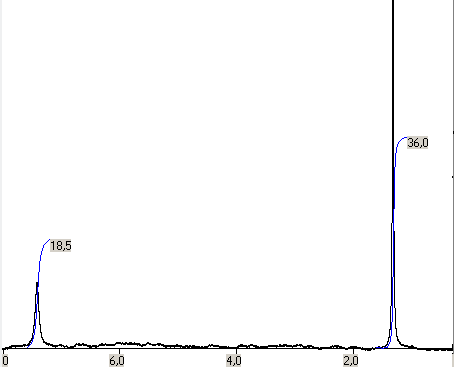
\includegraphics[width=0.6\linewidth]{pict1}
	\caption{ЯМР спектр на рабочей частоте 30 МГц}
	\label{fig:pict1}
\end{figure}

\begin{figure}[h]
	\centering
	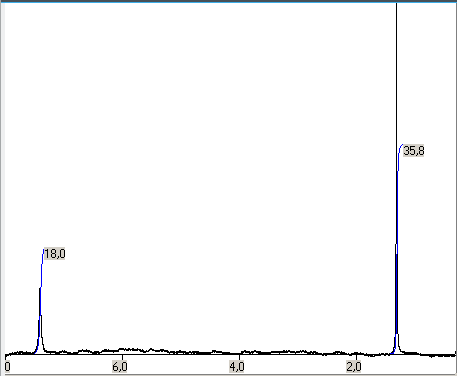
\includegraphics[width=0.6\linewidth]{pict2}
	\caption{ЯМР спектр на рабочей частоте 60 МГц}
	\label{fig:pict2}
\end{figure}

Приведу спектр для еще одной частоты. Качественный вид (количество неэквивалентных групп) сохраняется. При
дальнейшем повышении частоты сверхтонкое расщепление также не наблюдается, вплоть до увеличения значения постоянного магнитного поля до значения порядка $20$ Тл.

\begin{figure}[h!]
	\centering
	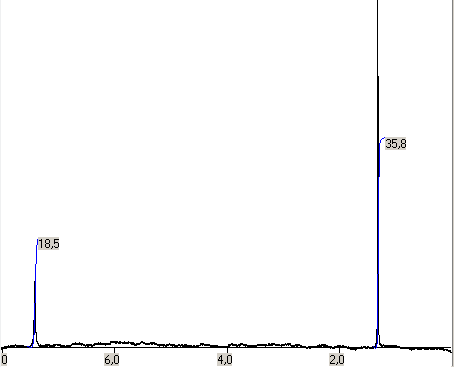
\includegraphics[width=0.6\linewidth]{pict3}
	\caption{ЯМР спектр на рабочей частоте 100 МГц}
	\label{fig:pict3}
\end{figure}

Соответствие резонансных частот и напряженностей постоянного магнитного поля представлю в таблице:

\begin{table}[h!]
	\caption{Зависимость $H_0$ от $\nu_0$}
	\label{table:1}
	\centering
	\begin{tabular}{|c|c|}
		\toprule
		Рабочая частота МГц &  Магнитное поле Тл  \\
		\midrule
		$30$  	&  0.71   \\
		$60$  	&  1.42   \\
		$100$ 	&  2.36   \\
		\bottomrule
	\end{tabular}
\end{table}

\begin{table}[h!]
	\caption{Зависимость величины химического сдвига от частоты для двух пиков соответственно}
	\label{table:2}
	\centering
	\begin{tabular}{|c|c|c|}
		\toprule
		Рабочая частота МГц & Химический сдвиг Гц & Химический сдвиг м.д.    \\
		\midrule
		$30$  	& $221 :: 40$  & $7.4 :: 1.3$ \\
		$60$  	&  $445 :: 75$ & $7.4 :: 1.4$ \\ 
		$100$ 	& $ 740:: 130$ & $7.4 :: 1.3$ \\
		\bottomrule
	\end{tabular}
\end{table}

Теперь мы наглядно видим преимущество использования шкалы в миллионных долях для химического сдвига.
Нас, прежде всего, интересует локальная электронная плотность возле атома водорода, и избавление от явной зависимости от рабочей частоты или напряженности магнитного поля позволяет соотносить результаты различных измерений.

\begin{table}[h!]
	\caption{Зависимость относительной интенсивности пиков от рабочей частоты}
	\label{table:3}
	\centering
	\begin{tabular}{|c|c|c|}
		\toprule
		Рабочая частота МГц & Отн. интенсивность левого пика & Отн. интенсивность правого пика    \\
		\midrule
		$30$  	& $18.5$  & $36.0$ \\
		$60$  	&  $18.0$ & $35.8$ \\ 
		$100$ 	& $ 18.5$ & $35.8$ \\
		Средние значения & $ 18.4$ & $35.9$ \\
		\bottomrule
	\end{tabular}
\end{table}

\newpage

Так как атомы водорода имеют спин $s = 1/2$ отношение интенсивностей будет целым числом. Из Таблицы $\ref{table:3}$ видно, что это отношение есть $18/36 = 1/2$. 

\subsection{Поиск решения обратной задачи ЯМР}


Мы имеем брутто-формулу $C10H14$.\\
Количество магнитно неэквивалентных групп равно двум.\\
Отношение интенсивностей в них $1/2$ соответственно.\\
Химический сдвиг $7.4$ и $1.3$ соответственно.\\

Видно, что не получается ровно разбить водород по интенсивности, значит будем пробовать ближайшие по количеству соотношения по водороду $4/10$ и $5/9$. С учетом химического сдвига плодотворным оказывается поиск в отношении $5/9$. 

\begin{figure}[h]
	\centering
	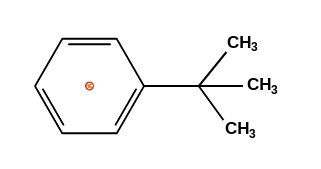
\includegraphics[width=0.6\linewidth]{pict4}
	\caption{Восстановленное по брутто-формуле соединение}
	\label{fig:pict4}
\end{figure}

Химический сдвиг эквивалентных групп хорошо соответствует характерным табличным значениям.

\subsection{Оценка относительной неоднородности постоянного магнитного поля}
Мы будим исходить из предположения о том, что шиммирование и вращение образца полностью исключают неоднородность поля.
Тогда нам следует измерить ширину пика с учетом шиммирования и вращения и без.
Возьмем рабочую частоту 30 МГц.\\
Без устранения неоднородности ширина большего по энергии пика $0.82\pm0.01$ Гц\\
C учетом шиммрования и вращения $0.48\pm0.01$ Гц\\

Тогда из соотношения \ref{eq2} можно заключить, что:

\begin{equation}
\label{eq3}
\frac{\delta\nu}{\nu_0} = \frac{\delta H}{H_0}
\end{equation}

Таким образом:

\begin{equation}
\label{eq4}
\delta H = \frac{\delta\nu}{\nu_0}H_0  
\end{equation}

Получаем оценку для неоднородности поля $\delta H \sim 10^{-11}  $\space Tл


